\documentclass[12pt, oneside]{report}

%\usepackage{ngerman}
\usepackage{latexsym}
\usepackage{amssymb}
\usepackage{mathrsfs}
%\usepackage{psfig}
\usepackage{graphicx}
\usepackage[latin1]{inputenc}
\usepackage{abschlussarbeit}
\usepackage{hyperref}
\usepackage{verbatim}
\usepackage{mathtools}
\usepackage{dsfont}
\usepackage{ulem}
\usepackage{color}
\usepackage{natbib}

%\usepackage[T1]{fontenc}
%\usepackage[english]{babel}
%\usepackage[ngerman]{babel}
%\usepackage{lmodern}
%\usepackage{pict2e}
%\usepackage{amsmath, amssymb, amstext, amsfonts, mathrsfs}
%\usepackage[squaren]{SIunits}
%\usepackage[latin1]{inputenc}
%\usepackage[ngerman]{babel}
%\usepackage{pict2e}
%\usepackage{graphicx}
%\usepackage{xcolor}
%\usepackage{amssymb}
%\usepackage{amstext}
%\usepackage{amsmath}
%\usepackage{txfonts}
%\usepackage{amsfonts}
%\usepackage{mathrsfs}
%\usepackage{fancybox}
%\usepackage{framed}
%\usepackage{hyperref}
%\usepackage{dsfont}


\bibliographystyle{abbrv}

\pagestyle{headings}
\bibliographystyle{plainnat}


\newtheorem{Algorithm}{Algorithm}
\newtheorem{Theorem}{Theorem}[section]
\newtheorem{Satz}{Satz}[section]
%% Ein sog. "Theorem" mit Abkuerzung "Satz" (das erste "Satz")
%% Das zweite "Satz" bezeichnet den Namen des Theorems. (z.B. "Satz x.y" erscheint im TeX-File).
%% [chapter] regelt die Numerierung der Saetze, in diesem Fall werden die Saetze pro Kapitel fortlaufend numeriert.
%
\newtheorem{Korollar}[Satz]{Korollar}
%% Hier haben wir ein "Theorem" mit Abkuerzung "Korollar", welches im Tex-File als "Korollar" erscheint und in die "Theorem"-Nummerierung
%% fortlaufend eingebunden wird (das "[Theorem]" bewirkt dies).
%\newtheorem{Proposition}[Satz]{Proposition}
%% Abkuerzung ist "Proposition", Name ist "Proposition", wird in "Theorem"-Nummerierung eingebunden.
%%Lemma, ebenfalls in "Theorem"-Nummerierung eingebunden
%\newtheorem{Lemma}[Satz]{Lemma}
%%Definition, ebenfalls in "Theorem"-Nummerierung eingebunden
\newtheorem{Definition}[Satz]{Definition}
%%Beispiel, ohne Nummerierung
%\newtheorem{Beispiel}{Beispiel}
\newtheorem{Example}{Example}
%%Annahme, nach Kapiteln nummeriert
%\newtheorem{Annahme}{Annahme}[chapter]
%% Labelnummerierung in 'roemisch'.
%\renewcommand{\labelenumi}{(\roman{enumi})}
\textwidth16cm
\textheight22cm

\topmargin0cm
\oddsidemargin0cm
\evensidemargin0cm



\pagestyle{headings}
%% enumerate equations by section, i.e. 5.6 for 6th eq. in section 5
\numberwithin{equation}{section}

\usepackage{mdframed}
\mdtheorem{mytheo}{OCP}
\usepackage{booktabs}% http://ctan.org/pkg/booktabs
\newcommand{\tabitem}{~~\llap{\textbullet}~~}

\newmdtheoremenv{algorithm}{Algorithm}


\begin{document}
\tableofcontents
% !TEX root = thesis.tex	
\chapter{Introduction}
\section{Motivation}
The goal of this thesis is...
\section{Traffic flow modelling}
Analyzing traffic flow has been an interdisciplinary research field of both mathematicians and civil engineers since the early 1950s. Over time different approaches for modelling traffic have been introduced and applied in extensive studies.
\begin{itemize}
	\item  On the \textbf{microscopic} scale every vehicle is considered as an individual agent whose dynamics are determined by the solution of an ordinary differential equation (ODE). The interaction between neighboring vehicles are usually based on simple equations and determine the behaviour of the collective. The most famous models of this approach are those of the \textit{follow-the-leader} kind \citep{Pipes.1953}. In those models the entire behaviour of the collective cars is fully determined by the one of the first car, namely the leader. Microscopic models can not only illustrate collective phenomena like traffic jams, but it can also be shown that under certain conditions the microscopic solution converges to the macroscopic solution as the number of vehicles approaches infinity \citep{E.Cristiani.}.
	\item \textbf{Mesoscopic} - or kinetic - models analyze transportation elements in small homogenous groups, where the probability of each group to be at time $t$ at location $x$ with velocity $v$ can be described by a function $f(t,x,v)$. This modelling approach requires the use of methods from statistical mechanics.
	\item \textbf{Macroscopic} models utilize the similarities of traffic flow and fluid dynamics. In those models the change of averaged quantities, like density, velocity etc., is described by means of partial differential equations (PDE). The oldest representative of macroscopic modelling are the LWR-models \citep{Richards.1956}, named after their inventors M. J. Lighthill, G. B. Whitham and P. I. Richards. Others include the Aw-Rascle model and the Payne-Whitham approach \citep{Aw.2000,Payne.1971}. For the rest of this thesis, this is the modelling approach of choice.
\end{itemize}
In macroscopic models the target is to analyze the change of measurable quantities. A typical quantity used in the analysis of traffic flow, analogous to fluid dynamics, is the density of mass. Let us denote the traffic density on a space interval $\left[x_1,x_2\right]$ at some time $t\in\mathbb{R}$ as $\rho(x,t)$, then we can write the total mass on this interval as 
\begin{equation}
	 \text{amount of cars }=\int_{x_1}^{x_2}\rho(x,t)dx
\end{equation}
For conserved quantities no mass is neither destroyed nor created. Therefore the mass on an interval can only change by inflowing and outflowing quantities. The quantity mass crossing the point $x$ at a time $t$ is given by the \textbf{traffic flux} $f:[0,\rho_{max}]\rightarrow[0,f^{max}]$. \newline 
\begin{figure}[h]
\center
\includegraphics[scale=0.4]{char_flux_upd}
\caption{Typical shape of the fundamental diagram of traffic flow}
\end{figure}
\newline
The traffic flux, or also referred to as \textit{fundamental diagram}, is typically assumed to follow the rule
\begin{equation*}
f'(\rho)\left(\sigma-\rho\right)>0
\end{equation*}
where 
\begin{equation*}
\sigma := \text{arg}\max_\rho f(\rho)
\end{equation*}
denotes the density where the maximum flux \begin{equation*}
f^{max} :=  f(\sigma)
\end{equation*}
is attained. \newline
Since the total mass on the global space interval is preserved, the rate of change of the mass on the interval $\left[x_1,x_2\right]$ is defined by the difference of the in- and outfluxes of the interval, e.g. \begin{eqnarray*}
	\frac{d}{dt}\int_{x_1}^{x_2}\rho(x,t)dx&=&f(\rho(x_1,t))-f(\rho(x_2,t))
\end{eqnarray*}
Rewriting this assuming differentiability of both functions $u$ and $f$ and integration over the time interval $\left[t_1,t_2\right]$ leads to:
\begin{equation}
\label{eq:integral_form}
	\int_{t_1}^{t_2}\int_{x_1}^{x_2}\frac{d}{dt}\rho(x,t)\ dx dt=\int_{t_1}^{t_2}\int_{x_1}^{x_2}\frac{d}{dx}\lbrace-f(\rho)\rbrace\ dx dt
\end{equation}
Assuming that $f$ is smooth, this leads the differential form of the \textbf{conservation law}:
\begin{equation}
\label{eq:conslaw}
\rho_t+(f(\rho))_x=0
\end{equation}
The LWR-model, as it will be the basis for the remaining thesis, assumes that the flux $f(\rho)=\rho(x,t)v(x,t)$ is linearly dependent on the velocity $v(x,t)$ of the wave at point $x$. In particular the flux used for the LWR-model can be written as
\begin{equation}
\label{eq:LWRflux}
f(\rho(x,t))=\rho(x,t)v_{max}\left(1-\frac{\rho(x,t)}{\rho_{max}}\right)
\end{equation}
where $u_{max}$ is the maximum density permitted by the road, and $v_{max}$ the maximum velocity obtainable by the wave.\newline
\newline
Other approaches like the Greenberg and Payne-Whitham model use highly nonlinear functions for their wave velocities, see \citep{May.1990,Payne.1971}.
\newline
\newline
Extending the conservation law \ref{eq:conslaw} with suitable initial conditions, we can formulate the full \textbf{Lighthill-Whitham-Richards model} as
\begin{eqnarray}
\rho_t+\left[v_{max}\rho(1-\frac{\rho}{\rho_{max}})\right]_x&=&0 \hspace{1cm} t>0\\
\rho(x,0)&=&\rho_0(x) \nonumber
\end{eqnarray}
\newline
The remaining thesis will be structured as follows: In chapter 2 we will extend the given LWR-model on a network of roads in order to be able to analyze urban traffic situations. We will also introduce the concept of buffers to guarantee the existence of unique solutions for the model. In chapter 3 we will discuss the numerical procedures in order to qualitatively simulate traffic flow computationally. Chapter 4 will deal with introduce the concept of traffic lights on the network. We will then propose two different optimization methods to control the light signals in order to maximize the flux on the network. The two approaches consist of a rather brute-force approach and a concept called model predictive control (MPC). The last chapter will then expand the model by the concept of pollution.
\newpage

% !TEX root = thesis.tex

\newpage
\chapter{The LWR model on networks}
So far we have only solved traffic flow problems on the real line. In order to analyze traffic flow more sophisticated problems under realistic scenarios, in particular in urban environments, it is necessary to extend the mathematical theory and the representation of traffic networks. The method of choice is hereby to represent traffic networks via directed graphs. This directed graph consists of a set of edges, representing the roads, and a set of nodes representing junctions. Every junction is thereby characterized by a finite number of incoming and a finite number of outgoing roads. 
\newline 
\newline
\section{Related literature}
Traffic flow on road networks has been a widely discussed topic over the past 70 years with an increasing interesent in the past century. 

\textbf{TODO:}
\begin{itemize}
\item summary of cummulative number pde, multi-path, garavello approach...
\end{itemize}
A much larger and well presented genealogy of the history of traffic flow modelling can be found in \citep{WageningenKessels.2015}.
\section{Basic principles of networks}
Rigorously we can define a network as followed, cf. \citep{Garavello.2006}:
\begin{Definition}
\label{network}
A network is a tuple $\left(\mathcal{N},\mathcal{E}\right)$, where $\mathcal{N}$ is a finite collection of vertices, and $\mathcal{E}$ a finite collection of $n_R$ edges, where every node represents a junction and every edge represents a unidirectional road. Each road $e_i=\left[a_i,b_i\right]\in\mathbb{R}, i=1...n_R$ is defined over a real interval. 
\end{Definition}
We further require the following properties:
\begin{itemize}
\item[1)]Every junction $J\in\mathcal{N}$ defines a union of two non-empty sets $\delta^{in}(J)$ and $\delta^{out}(J)$ where $\delta^{in}(J),\delta^{out}(J)\subset\mathcal{E}$, representing incoming and outgoing roads of the junction $J$, respectively.
\item[2)\label{item}] For junctions $I,J\in\mathcal{N}, I\neq J$ we require $\delta^{in}(I)\cap \delta^{in}(J)=\emptyset$ and $\delta^{out}(I)\cap \delta^{out}(J)=\emptyset$ 
\item[3)] \label{edges} If $e_i\not\in\bigcup_{J\in\mathcal{N}}\delta^{in}(J)$ then $b_i=\infty$. In this case $e_i\in\mathcal{E}^{out}$ where $\mathcal{E}^{out}$ denotes the set of all outgoing roads for the network. Furthermore if $e_i\not\in\bigcup_{J\in\mathcal{N}}\delta^{out}(J)$ then $a_i=-\infty$. In this case $e_i\in\mathcal{E}^{in}$ where $\mathcal{E}^{in}$ denotes the set of all incoming roads for the network.
\end{itemize}
These assumptions guarantee that the resulting network is indeed a valid graph. Requirement 1) implies that every road starts and ends in at most one junction. Requirement 2) then says that if a road does not start (end) at a junction then it is considered as an inflow (outflow) of the network. \newline
\newline
Another method to represent a road network is via so-called \textbf{adjescency matrices} \citep{Biggs.1993}.
\begin{Definition}
\label{adjesM}
Let $\mathcal{N}$ be a set of edges with $|\mathcal{N}|=n_R$. Then the adjescency matrix is a square $n_R\times n_R$-matrix $A$ with \begin{equation*} 
A_{ij} = \bigg\{\begin{array}{ll}
	1 & \text{if there exists a junction between road} \ e_j \ \text{and} \ e_i \\
	0 & \text{else}
\end{array}
\end{equation*}
\end{Definition}
The adjescency matrix stores information if there is a direct connection between road $e_j$ and $e_i$. \newline
\newline
\underline{\textbf{Remark:}} \newline
Having given the network as in definition \ref{network} one can easily derive the corresponding adjescency matrix as in definition \ref{adjesM}, and vice versa. \textbf{BEING MORE SPECIFIC??? also about problem of non-unique indexing of junctions?}
\begin{Example}
Let us consider network displayed in figure \ref{fig:network_ex}. Then the corresponding adjescency matrix can be written as
\begin{equation*}
A=\left(\begin{array}{ccccc} 0 & 0 & 0 & 0 & 0\\0 & 0 & 0 & 0 & 0\\1 & 1 & 0 & 0 & 0\\0 & 0 & 0 & 0 & 0\\0 & 0 & 1 & 1 & 0
\end{array} \right)
\end{equation*}
\end{Example}
\begin{figure}[h]
\center
\includegraphics[scale=0.3]{example_network}
\caption{Example of a network\label{fig:network_ex}}
\end{figure}
\section{Modelling on networks - the buffer model}
\label{buffer_model}
\underline{\textbf{The setting:}} \newline
\newline
Consider a family of $n+m$ roads, all joining at a single junction. The indices $i\in\{1,...,m\}=:\mathcal{I}$ hereby denote \textit{incoming roads} and indices $j\in\{m+1,...,m+n\}=:\mathcal{O}$ denote \textit{outgoing roads}. Then the evolution of the density of cars $\rho_k(x,t)$ on the $k-th$ road can be described by the \textbf{conservation law}
\begin{subequations}
\label{conslaw}
\begin{equation} 
	(\rho_k)_t+f(\rho_k)_x=0.
\end{equation}
accompanied by intial densities $\rho_k(x,0)=\rho_{k,0}(x)$ and external inflows into the network defined by 
\begin{equation}
f(\rho_k(a_k,t)=q_k(t) \hspace{0.4cm} \forall e_k\in\mathcal{E}^{in}
\end{equation}
Furthermore the corresponding inflows and outflows of the junctions are given as
\begin{eqnarray}
	f(\rho_k(b_k,t))=\bar{f_k}(t) & \forall e_k\in\mathcal{E}\setminus\mathcal{E}^{out} \\
	f(\rho_k(a_k,t))=\hat{f_k}(t) & \forall e_k\in\mathcal{E}\setminus\mathcal{E}^{in}
\end{eqnarray}
where the junctions fluxes $\bar{f_k}$ and $\hat{f_k}$ are defined later. \newline
For the roads leaving the network we also impose Dirichlet boundary conditions.
\end{subequations}
\newline
\newline
\underline{\textbf{The model}} \newline
\newline
In order to be useful for the analysis of global optimization, the used traffic flow model at junctions should provide two crucial properties:
\begin{itemize}
\item Well posedness for $\mathcal{L}^\infty$ data
\item Continuous solution w.r.t. weak convergence
\end{itemize} 
Due to the ill-posedness of the general junction model in \citep{Garavello.2006} for certain input data, we need to come up with a different approach. \newline
\newline
In \citep{Bressan-Conservation} a model is proposed where each intersection in the model includes a \textbf{buffer} with limited capacity. The current filling level of the buffer in front of the outgoing road $j\in\mathcal{O}$ may be denoted as the \textit{queue length} $q_j\left(t\right)$. The rate of flux at which cars from incoming roads enter the intersection is controlled by the current length of the queues. The outgoing fluxes are governed by the queue length and the personal preference destination of the individual drivers, as well as the maximum permitted fluxes on the designated roads. \newline
\newline
The main results of their analysis can be stated as:
\begin{itemize}
\item[I.] If the queue lenghts $q_j$ for every outgoing road are given, the initial boundary value problems on each road become decoupled and can be solved individually, first on every incoming road, and secondly on every outgoing road. The densities $\rho_k(t,x)$ on every road $k=1...m+n$ can then be explicitly computed via a Lax type formula.
\item[II.] Given the densities, the lenghts $q_j$ of the queues can be determined by balancing the influxes and outfluxes of the intersection. The queue lengths can finally be obtained as a fixpoint of a contractive transformation $q\rightarrow\Delta(q)$ where $q$ needs to be Lipschitz continuous.
\item[III.] The buffer model is thus well-posed at intersections for general $\mathcal{L}^\infty$ data. It is also shown that the traffic flow model is continous w.r.t. weak convergence.
\end{itemize}
The interested reader is referred to \citep{Bressan-Conservation} for the proofs.
\newline
\newline
\newline
Let the general setting be as earlier in this section. Further we include two realistic assumtions for the boundary values at the entrance and exit points of junctions:
\begin{itemize}
\item[i.] \textbf{Driver's preferences $\Theta_{i,j}$} define the fraction of cars on road $i$ that want to exit the junction in direction of road $j$. \\
	\[\Theta_{i,j}\in\left[0,1\right]\]
\item[ii.] \textbf{Relative priorities $\eta_i$ given to incoming roads} e.g. external effects like traffic lights
\end{itemize}
For every junction $J$ we can define the driver's preferences $\Theta$, i.e. the percentage of drivers going from one incoming to out outgoing road, as followed:
\begin{Definition}{}
Given a junction $J$ with $n:=|\delta^{in}(J)|$ incoming roads, say $e_1,...,e_n$, and $m:=|\delta^{out}(J)|$ outgoing roads, say $e_{n+1},...,e_{n+m}$. Then the traffic distribution matrix $\Theta$ is given by 
\begin{equation}
\Theta=\left(\begin{array}{ccc}
	\Theta{n+1,1} & \cdots & \Theta{n+1,n} \\
	\vdots & \ddots & \vdots \\
	\Theta{n+m,1} & \cdots & \Theta{n+m,n}
\end{array}\right)
\end{equation}
where $0\leq \Theta_{i,j}\leq 1$ for every $i=1,...,n$ and $j=n+1,...,n+m$. Furthermore we impose the validity condition
\[\Theta_{i,j}\in\left[0,1\right], \hspace{1cm}\sum_{j\in\delta^{out}(J)}\Theta_{i,j}=1\]
\end{Definition}
In general, $\Theta_{i,j}=\Theta_{i,j}(t,x)$ needs not to be necessarily constant, but can be time- and location-dependent. In the following it is assumed that the drivers' preferences are known in advance and that they do not change their itinerary throughout the network. Then the conservation law reads
\[(\Theta_{i,j}\rho_i)_t+[\rho_i\Theta_{i,j}v(\rho_i)]_x=0\]
Using product rule and reordering yields
\[\rho_i[(\Theta_{i,j})_t+v(\rho_i)(\Theta_{i,j})_x]+\Theta_{i,j}[(\rho_i)_t+(\rho_iv(\rho_i))_x]=0\]
The second term vanishes as the general conservation law still needs to be fulfilled. For zero density on the road this is fulfilled trivially. For $\rho_i\neq 0$ we obtain the passive scalar transport equation along the flux:
\begin{equation}
(\Theta_{i,j})_t+v(\rho_i)(\Theta_{i,j})_x=0
\end{equation}
A similar approach has been persued by \citep{Bressan.2013}. In their intersection model the capacity of the queues is arbitrarily big. Cars wanting to ender road $j$ but exceed the maximum outflux of the intersection are instead stored in the queue. As a consequence there is no backward propagation of queues and therefore no emergence of shocks on incoming roads. \newline
\newline
The model by \citep{Bressan-Conservation} extends this model. Consider a single junction and let $M>0$ be the maximum capacity of the queue. Then the incoming fluxes into the junction depend on the current degree of occupancy of the buffer, which is defined by 
\[q=(q_j)_{j\in\mathcal{O}},\hspace{1cm}q\in\mathbb{R}^n\]
The Cauchy problem for traffic flow on a network can thus be formulated as
\begin{eqnarray*}
(\rho_i)_t+f_i(\rho_i)_x&=&0 \\
(\Theta_{ij})_t+v(\rho_i)(\Theta_{i,j})_x&=&0
\end{eqnarray*}
supplemented by suitable initial conditions.\newline
\newline
The \textbf{maximum fluxes} that can enter and exit the intersection depend on the current filling level on the incoming and outgoing road, respectively. In particular they are given by the following equations.
\begin{itemize}
	\label{eg:maxfluxes}
	\item Maximum fluxes on incoming roads: \[\omega_i(\rho):=\begin{cases}
		f(\rho) & \rho\leq\sigma \\
		f(\sigma) & \rho>\sigma \end{cases}
	\]
	\item Maximum fluxes on outgoing roads: \[\omega_j(\rho):=\begin{cases}
		f(\sigma) & \rho\leq\sigma \\
		f(\rho) & \rho>\sigma
	\end{cases}\]
\end{itemize}	
This property ensures that Riemann problems on incoming roads are solved by waves with negative speed, and Riemann problems on outgoing roads are solved by waves with positive speed. \newline
\newline
Based on the junctions fluxes, we can also derive the rate of change of the size of the junction buffer. In detail, conservation of mass yields the additional differential equation for the \textbf{evolution of the queue size}
\begin{equation}
\label{eq:queue}
\dot{q_j}=\sum_{i\in\mathcal{I}}\bar{\Theta}_{i,j}\bar{f_i}-\bar{f_j}
\end{equation}
where $\bar{f_j}$ denote the boundary fluxes at the junction, $k\in\mathcal{I}\cup\mathcal{O}$. \newline
\newline
We are now ready to state two sets of equations regarding the incoming and outgoing junction fluxes depending on the drivers' choices $\Theta_{ij}$ and the queue lenghts $q_j$. \newline \newline
%SBJ
The first model provides a shared buffer of capacity $M$ for every outgoing junction. Incoming cars can cross the intersection governed by the amount of free space left in the queue, regardless of the car's destination. Once within the junction, cars leave at the maximum rate allowed by the outgoing road of their choice.
\newline \newline
\textbf{Single Buffer Junction model (SBJ):} Consider a constant $M>0$, describing the maximum capacity of the junction at any given time, and constants $c_i>0, i\in\mathcal{I}$ accounting for priorities given to the differnt incoming roads. \newline
We then require that the incoming fluxes $\bar{f}_i$ satisfy
\begin{subequations}
\label{{eq:sbj}}
\begin{equation}
\bar{f}_i=\min\lbrace \omega_i,c_i(M-\sum_{j\in\mathcal{O}}q_j)\rbrace, \hspace{1cm} i\in\mathcal{I}\end{equation}
Furthermore, the outgoing fluxes $\hat{f}_j$ should satisfy
\begin{equation}\hat{f}_j=\Bigg\lbrace\begin{array}{ll}
	\omega_j & q_j>0 \\
	\min\lbrace\omega_j, \sum_{i\in\mathcal{I}}\bar{f}_i\bar{\Theta}_{i,j}\rbrace & q_j=0

\end{array}\end{equation}
\end{subequations}
As seen, the outgoing fluxes are uniquely defined once the incoming fluxes are known in addition to the current status of the queue.
\newline
\newline
The second model uses $n$ different buffers, one for every outgoing road. Once having entered the junction, cars are admitted to their desired road of destination depending on the length of the queue in front of the desired road.
\newline
\newline
\textbf{Multiple Buffer Junction model (MBJ):} Consider constants $M_j>0, j\in\mathcal{O}$, describing the maximum capacitis of the buffers in front of the $n$ outgoing roads of the junction at any given time, and constants $c_i>0, i\in\mathcal{I}$ accounting for priorities given to the differnt incoming roads. \newline
We then require that the incoming fluxes $\bar{f}_i$ satisfy
\[\label{eq:mbj}\bar{f}_i=\min\lbrace \omega_i,\frac{c_i(M_j-q_j)}{\Theta_{i,j}},j\in\mathcal{O}\rbrace, \hspace{1cm} i\in\mathcal{I}\]
Furthermore, the outgoing fluxes $\hat{f}_j$ should satisfy
\[\hat{f}_j=\Bigg\lbrace\begin{array}{ll}
	\omega_j & q_j>0 \\
	\min\lbrace\omega_j, \sum_{i\in\mathcal{I}}\bar{f}_i\bar{\Theta}_{i,j}\rbrace & q_j=0

\end{array}\]
Now we can define the full \textbf{buffer model} by Bressan et al. \citep{Bressan-Conservation}
\begin{eqnarray}
(\rho_i)_t+f_i(\rho_i)_x&=&0 \hspace{1cm},e_i\in \mathcal{E} \\
\dot{q_j}&=&\sum_{i\in\mathcal{I}}\bar{\Theta}_{i,j}\bar{f_i}-\bar{f_j} \nonumber\\
f(\rho_k(a_k,t)&=&q_k(t) \hspace{1cm}\forall e_k\in\mathcal{E}^{in} \nonumber\\
f(\rho_k(b_k,t))&=&\bar{f_k}(t)  \hspace{1cm}\forall e_k\in\mathcal{E}\setminus\mathcal{E}^{out} \nonumber\\
	f(\rho_k(a_k,t))&=&\hat{f_k}(t) \hspace{1cm}\forall e_k\in\mathcal{E}\setminus\mathcal{E}^{in} \nonumber
\end{eqnarray}
with external inflows $q_k(t)$ and junctions fluxes $\bar{f_k}(t)$ and $\hat{f_k}(t)$ as defined in \eqref{eq:sbj}
\newline
\newline
\textbf{Limitations of this approach:} \begin{itemize}
\item This approach focuses on maximizing the flux of mass through the junction. A counter-intuitive effect of this approach is the following:
\item Consider a trivial junction at $x=0$ with one incoming and one outgoing road and initial data $\rho_{in}>\sigma$ and $\rho_{out}=0$. Then the result won't be continuous at $x=0$. In particular the outgoing flux will be $f^{max}=f(\sigma)$, hence $\rho(0^+,t)=\sigma$ whereas $\rho(0^-,t)>\sigma$ by assumption.
\end{itemize}
% !TEX root = thesis.tex

\newpage
\chapter{Numerical approximations}
In order to solve conservation laws of the form \eqref{eq:conslaw} we usually assume smooth initial conditions $\rho(x,0)$. We are naturally interested in the difficulties caused by discontinuities in the solution. Straight-forward numerical methods like the finite difference approximation usually have difficulties near the discontinuity. Consider for instance the scalar (linear) advection equation 
\begin{eqnarray}
\label{eq:advection}
&u_t+Au_x=0, \hspace{0,5cm} -\infty<x<\infty, t\geq 0 \nonumber \\
&u(x,0)=\begin{cases} 1 \hspace{0,5cm} x<0\\ 0  \hspace{0,5cm} x>0 \end{cases}  
\end{eqnarray}
Obviously the analytical solution obtained by the method of characteristics is given by a travelling show wave $u(x,t)=u_0(x-At)$ with wave speed $A$.
\textcolor{red}{ADD Lax Equivalence Theorem?? }
Unfortunately the finite difference approach is inconsistent, as the finite difference approximation to $u_x$ at the discontinuity $x=0$ will not approach 0, e.g.
\begin{equation*}
	u_x\sim\frac{u_0(At+h)-u_0(At-h)}{2h}=\frac{0-1}{2h}\rightarrow-\infty, \text{ as } h\rightarrow 0
\end{equation*}
In particular, the \textit{local truncation error} 
\begin{equation}
L_k(0,t):=\frac{1}{k}\left[u(0,t+k)-u(0,t)\right]-a\frac{u_0(At+h)-u_0(At-h)}{2h}
\end{equation}
for the finite difference scheme does not vanish for $h,k\rightarrow 0$ (see also \citep{LeVeque.1992}). A numerical method of \textbf{order p} fulfills that $L_k(x,t)=\mathcal{o}(k^p)$. This means that the finite difference scheme for discontinuous data does neither provide local nor global convergence towards the analytical solution. \newline
\newline
For linear systems of the form \eqref{eq:advection} a wide variety of convergent numerical methods using adjusted finite difference schemes are given. Some possibilites are stated in Table \ref{schemes}. 
\begin{table}[h]
\renewcommand{\arraystretch}{2}%
\begin{tabular}{|l|l|c|}
\hline  
Name & Difference equation & Order  \\ \hline
Lax-Friedrich & $\begin{array}{lcl}
u(x,t+k)&=&\frac{1}{2}\left(u(x+h,t)+u(x-h,t)\right) \\
&-&\frac{k}{2h}A(u(x+h,t)-u(x-h,t))
\end{array}$ & 1\\
Upwind $(A>0)$& $\begin{array}{lcl}u(x,t+k)&=&u(x,t)-\frac{k}{2h}A(u(x,t)-u(x-h,t))\end{array}$ & 1 \\
Lax-Wendroff & $\begin{array}{lcl}
u(x,t+k)&=&u(x,t)-\frac{k}{2h}A(u(x+h,t)-u(x-h,t)) \\
&+&\frac{k^2}{2h^2}A^2\left(u(x+h,t)-2u(x,t)+u(x-h,t)\right)
\end{array}$ & 2 \\
Beam-Warming & $\begin{array}{lcl}
u(x,t+k)&=&u(x,t)-\frac{k}{2h}A(3u(xh,t)-4u(x-h,t) \\
&+&u(x-2h,t))+\frac{k^2}{2h^2}A^2((u(xh,t)\\&-&2u(x-h,t)+u(x-2h,t))
\end{array}$ & 2 \\
\hline
\end{tabular}
\caption{\label{schemes}Finite difference schemes for the linear advection problem \eqref{eq:advection}.}
\end{table}
First order method (Upwind, Lax-Friedrich) typically produce a flattened solutions compared to the original solutions, whereas second order methods (Lax-Wendroff and Beam-Warming) give oscillations. These phenomena are displayed in Figure \ref{fig:schemes}. 
\begin{figure}[h]
\center
\includegraphics[scale=0.4]{numeric_schemes}
\caption{\label{fig:schemes} Numerical and exact solution of conservation law \eqref{eq:advection}} at $t=0.5$ and step size $h=0.0025$ using the following methods (top left to bottom right) (a) Lax-Friedrich, (b) Upwind, (c) Lax-Wendroff, (d) Beam-Warming
\end{figure}
\section{The Godunov scheme for nonlinear conservation laws}
Finite difference schemes as discussed in the introductive part of this chapter provide \textit{smooth} solutions, even if the initial datum of the conservation law contains discontinuities and jumps. Even to nonlinear problems these PDEs can often be linearized and therefore results from the linear FD methods applied in order to obtain convergence results for nonlinear problems \citep{Strang}. There are several limitations to this approach: \newline Firstly it is not guaranteed that the obtained numerical solution really converges towards the analytical discontinuous solution (see e.g. Burger's equation). Secondly the modelling of travelling waves, in particular the evolution of traffic jams and shocks often emerge from initial discontinuities discontinuities. Thus a different approach has to be persued. \newline
\subsection{Theory of conservative numerical schemes}
Let us consider the x-t-plane as the operating space. We can discretize this space by choosing a mesh with step size $h:=\Delta x$ and time step $k:=\Delta t$, $\frac{h}{k}=C>0$ fixed. In particular the mesh points are given by
\begin{eqnarray*}
	x_j&=&jh, \hspace{1cm} j=\dots,-1,0,1,\dots \\
	t_n&=&nk, \hspace{1cm} n=0,1,\dots
\end{eqnarray*}
We also define the midpoints in space 
\begin{equation*}
	x_{j\pm\frac{1}{2}}:=x_j\pm\frac{h}{2}
\end{equation*}
We can now define the \textbf{cell averages} of the density $\rho(x,t)$ on the mesh as
\begin{equation}
u_j^n:=\int_{x_{j-\frac{1}{2}}}^{x_{j+\frac{1}{2}}}\rho(x,t_n)dx
\end{equation}
The idea of the \textbf{Godunov scheme} is to approximate the solution $\rho(x,t_n)$ to conservation law \eqref{eq:integral_form} by a piecewise constant function 
\begin{equation}
u^n(x,t_n)=u_j^n \hspace{1cm} \text{if} \ x_{j-\frac{1}{2}}\leq x < x_{j+\frac{1}{2}}
\end{equation}
 and by solving the Riemann problems caused by the space discretization on the time interval $[t_n,t_{n+1}]$. 
Following from the integral form of conservation law \eqref{eq:integral_form}, namely
\begin{eqnarray}
\int_{x_{j-\frac{1}{2}}}^{x_{j+\frac{1}{2}}}\rho(x,t_{n+1})dx &=& \int_{x_{j-\frac{1}{2}}}^{x_{j+\frac{1}{2}}}\rho(x,t_{n})dx \\
&&-\left[\int_{t_{n}}^{t_{n+1}}f(\rho(x_{j+\frac{1}{2}},t))dt-\int_{t_{n}}^{t_{n+1}}f(\rho(x_{j-\frac{1}{2}},t))dt\right] \nonumber
\end{eqnarray}
we obtain \begin{equation}
\label{eq:conservative}
u_j^{n+1}=u_j^n-\frac{1}{h}\left[\int_{t_{n}}^{t_{n+1}}f(\rho(x_{j+\frac{1}{2}},t))dt-\int_{t_{n}}^{t_{n+1}}f(\rho(x_{j-\frac{1}{2}},t))dt\right]
\end{equation}
with the \textbf{numerical flux function} 
\begin{equation}
\label{eq:num_flux}
F(u_j^n,u_{j+1}^n)\sim \frac{1}{k}\int_{t_n}^{t_{n+1}}f(\rho(x_{j+\frac{1}{2}},t)dt
\end{equation}
which plays the role of the average flux through $x_{j+\frac{1}{2}}$ over the time interval $[t_n,t_{n+1}]$. Numerical methods of the form \eqref{eq:conservative} are called \textit{in conservative form} as they still fulfill the conservation law. 
\newline
\newline
We also note that in practise equation \ref{eq:num_flux} simplifies since $u_j^n$ at point $x_{j+\frac{1}{2}}$ is constant along the line $[t_n,t_{n+1}]$ (also see picture \textcolor{red}{ADD picture like LeVeque p.139}.  Therefore the numerical flux at point $x_{j+\frac{1}{2}}$ only depends on the neighboring densities $u_j^n$ and $u_{j+1}^n$. Denoting this value by $u^*(u_j^n,u_{j+1}^n$ the numerical flux reduces to
\begin{equation}
F(u_j^n,u_{j+1}^n)=f(u^*(u_j^n,u_{j+1}^n))
\end{equation}
Obviously the scheme is consistent, since $F(u_j^n,u_{j}^n)=f(u_j^n))$. \newline
We mentioned earlier that $u_j^n$ at $x_{j+\frac{1}{2}}$ is constant along the line $[t_n,t_{n+1}]$. This only holds if the cells are "small enough" such that two shocks resulting from neighboring Riemann problems do not interact between two time steps. As the wave speed is bounded by the eigenvalue of $f'(u)$ we require that \begin{equation}
c_C:=\frac{k}{h}|\sup(f'(u))|\leq 1
\end{equation} 
$c_C$ is also called the Courant-number and serves as the one-dimensional CFL-condition \citep{Courant.1928}.
\newline
\newline
The \textbf{Godunov method} now consists of seperately solving every Riemann problem between every two neighboring cells. Let $u_j$ and $u_{j+1}$ be the densities on two neighboring cells. Then the flux $f(u^*(u_j,u_{j+1})$ is given by
\begin{equation}
\label{eq:numerical_flux}
f(u^*(u_j,u_{j+1}))=\begin{cases} \min \left[f(u_j),f(u_{j+1})\right] \hspace{1cm}\text{if} \ u_l\leq u_r \\
%f(\sigma)\hspace{1cm}\text{if} \ u_r\leq\sigma\leq u_l \\
%f(u_r) \hspace{1cm}\text{if} \ \sigma\leq u_r \leq u_l \\
%f(u_l) \hspace{1cm}\text{if} \  u_r\leq u_l\leq\sigma
\max \left[f(u_j),f(u_{j+1})\right] \hspace{1cm}\text{if} \ u_l\geq u_r
\end{cases}
\end{equation}
This form of the resulting flux function is valid for any general scalar conservation laws, even for nonconvex fluxes.
In the convex case we can distinguish 4 cases for the numerical flux \eqref{eq:numerical_flux}, see Figure \ref{fig:solution_types}:
\begin{enumerate}
\item $f'(u_j),f'(u_{j+1})\geq 0$: Here the solution consists of a rarefaction wave with $u^*(u_l,u_r)=u_j$.
\item $f'(u_j),f'(u_{j+1})\leq 0$: The solution consists of a rarefaction wave with $u^*(u_l,u_r)=u_{j+1}$.
\item $f'(u_{j+1})<0\leq f'(u_j)$: Then there is a shock through $x_{j+\frac{1}{2}}$ and \begin{equation*}
u^*(u_j,u_{j+1})=\begin{cases} u_j &: s\geq 0 \\
u_{j+1} &:s<0\end{cases}
\end{equation*}
with the shock speed \begin{equation*}
s=\frac{f(u_{j+1})-f(u_j)}{u_{j+1}-u_j}
\end{equation*}
\item $f'(u_{j+1})>0\geq f'(u_j)$: In this case we have the so-called transonic rarefaction wave and $u^*(u_j,u_{j+1})=\sigma$, with $u=\sigma$ the unique point at which $f'(u)=0$ (cf. \eqref{eq:max_flux}).
\end{enumerate}
\begin{figure}[h]
\center
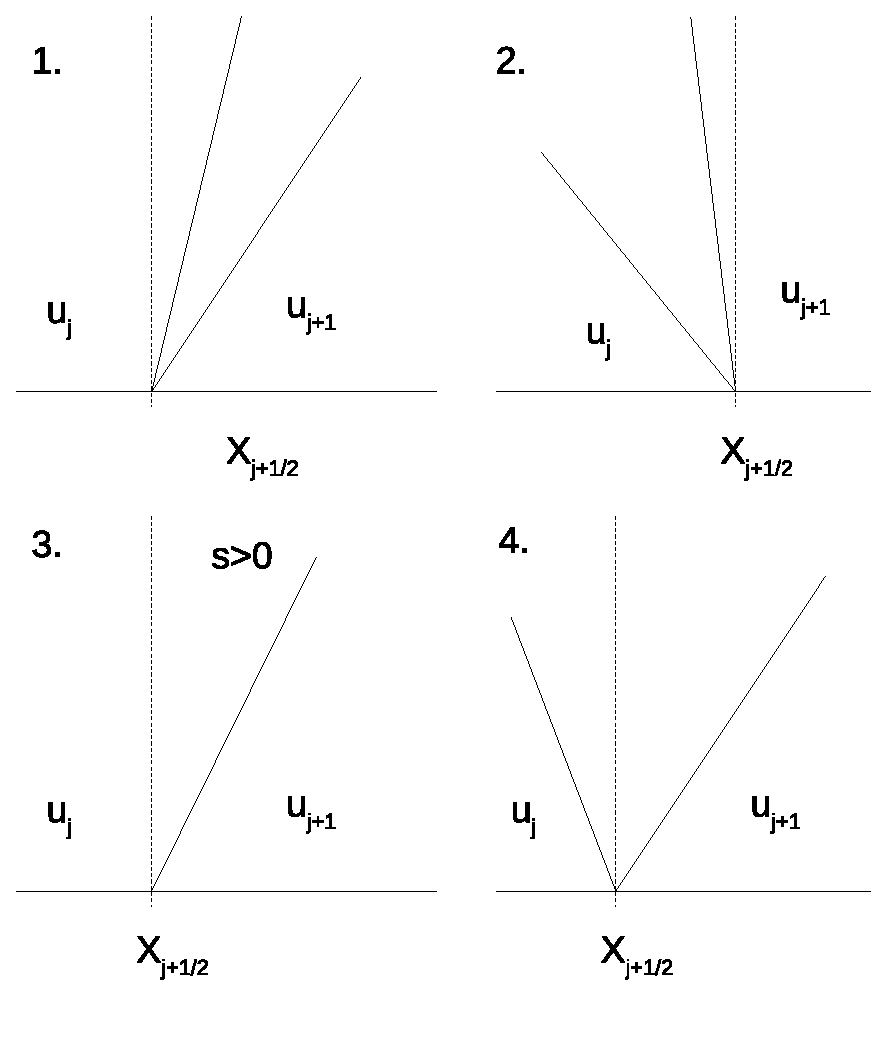
\includegraphics[scale=0.6]{figures/solution_types}
\caption{\label{fig:solution_types} Different types of solutions for the Riemann problem dependent on densities $u_j^n$ and $u_{j+1}^n$.}
\end{figure} \newline
\newline
In the following we want to apply the Godunov scheme on the buffer model defined in section \ref{buffer_model}.
\subsection{The Godunov scheme for the buffer model}
Let us consider an arbitrary connected road network $(\mathcal{N},\mathcal{E})$ with $n_R$ roads and $n_J$ junctions. On every road $e_i=[a_i,b_i]$ we apply the discretization $x_{i,j}=a_{i,jh}, j=0,...,D_i, x_{i,D_ih}=b_i$, with $D_i=\frac{b_i-a_i}{h}-1$ the number of cells on road $e_i$. Let us then denote $u_{i,j}^n$ the density on the j-th cell of road $e_i$ at time $t=nk$.\newline
\newline
We can now define on all \textit{inner cells} of every road $e_i$ the Godunov scheme 
\begin{subequations}
\label{eq:Godunov}
\begin{equation}
u_{i,j}^{n+1}=u_{i,j}^n-\frac{k}{h}\left[f(u^*(u_{i,j}^n,u_{i,j+1}^n))-f(u^*(u_{i,j-1}^n,u_{i,j}^n))\right],\hspace{1cm} e_i\in\mathcal{E}, j=1,\dots,D_i-1
\end{equation}  
We incorporate the \textit{externally inflowing densities} $q_i(t), e_i\in\mathcal{E}^{in}$ by introducing a ghost cell at the beginning of each road $e_i$. Then we define 
\begin{equation}
u_{i,0}^{n+1}=u_{i,0}^n-\frac{k}{h}\left[f(u^*(u_{i,0}^n,u_{i,1}^n)-f(u^*(v_{i,1}^n,u_{i,0}^n)) \right], \hspace{1cm} i\in\mathcal{E}^{in}
\end{equation} 
with the inflowing density $v_{i,1}^n:=\int_{t_n}^{t_{n+1}}\rho_{in,i}(t)dt$. \newline
The outfluxes leaving the network can be treated analogously. \newline
\newline
For junctions we recall equations \eqref{eq:sbj} for the junction fluxes in the single buffer model. Accordingly, we define for roads coming into junction $J$
\begin{equation}
u_{i,D_i}^{n+1}=u_{i,D_i}^n-\frac{k}{h}\left[\bar{f}_i-f(u^*(u_{i,D_i-1}^n,u_{i,D_i}^n)) \right], \hspace{1cm} i\in\delta^{in}(J)
\end{equation}
For outgoing roads of junction $J$ we analogously define the scheme
\begin{equation}
u_{i,0}^{n+1}=u_{i,0}^n-\frac{k}{h}\left[f(u^*(u_{i,0}^n,u_{i,1}^n))-\hat{f}_i \right], \hspace{1cm} i\in\delta^{out}(J)
\end{equation}
\end{subequations}
\underline{\textbf{Remarks:}}\begin{itemize}
\item For the computation of the buffer, which is needed for the junction fluxes, we use a simple difference quotient to approximate $\dot{q}$,
\begin{equation}
	q_j^{n+1}=q_j^n+k\left[\sum_{i\in\delta^{in}(J)}\bar{\Theta}_{i,j}\bar{f_i}-\bar{f_j}\right], \hspace{1cm}J\in\mathcal{N},j\in\delta^{out}(J)
\end{equation}
\item For convenience we condense equations \eqref{eq:Godunov}a-d on road $e_i$ to the condensed Godunov scheme 
\begin{equation}
u_i^{n+1}=G(u_i^n)
\end{equation}
\end{itemize} 
\section{Examples}

% !TEX root = thesis.tex
\chapter{Traffic light optimization}
As discussed in section \ref{buffer_model} we can model external effects, especially traffic lights, by assigning relative priorities \[\eta_i\in\left[0,1\right] , \hspace{1cm} e_i\in\mathcal{E}\setminus\mathcal{E}^{out}\] to roads prior to intersections. These values have the effect that only a fraction of the flux $\bar{f_i}$ as defined in the buffer model can enter the junction and pass it towards outgoing roads. In particular the binary values $\eta_i=1$ and $\eta_i=0$ for road $e_i$ correspond to green and red phases, respectively, for the particular incoming road. \newline \newline
For every junction $J$ the \textbf{feasibility condition} must hold. It is given by
\begin{equation}
\label{eq:feasibility}
\sum_{e_i\in\delta^{in}(J)}\eta_i(t)=1
\end{equation}
assuring that cars from only one road can cross the junction at any time $t$. \newline
\newline
This leads to a necessary update of the junction fluxes. In detail we define the \textbf{influx under applied traffic control} as
\begin{equation}
\label{eq:control_in}
\bar{\bar{f_k}}(t,\eta_k):= \min\lbrace \omega_k,c_k(M-\sum_{j\in\mathcal{O}}q_j)\rbrace\cdot \eta_k(t)
\end{equation}
The corresponding \textbf{outflux under applied traffic control} is given by
\begin{equation}
\label{eq:control_out}
\hat{\hat{f_j}}(t,\eta):=\Bigg\lbrace\begin{array}{ll}
	\omega_j & q_j>0 \\
	\min\lbrace\omega_j, \sum_{i\in\mathcal{I}}\bar{\bar{f_i}}\bar{\Theta}_{ij}\rbrace & q_j=0
\end{array}
\end{equation}
For the conservation law 
\begin{subequations}
\label{basic_conslaw}
\begin{eqnarray}
	(\rho_k)_t+f(\rho_k)_x&=&0  \hspace{0.5cm}\forall e_k\in\mathcal{E}\\
	f(\rho_k(b_k,t))&=&\bar{\bar{f_k}}(t) \hspace{0.5cm}\forall e_k\in\mathcal{E}\setminus\mathcal{E}^{out}	\\
	f(\rho_k(a_k,t))&=&\hat{\hat{f_k}}(t) \hspace{0.5cm}\forall e_k\in\mathcal{E}\setminus\mathcal{E}^{in}
\end{eqnarray}
\end{subequations} 
with junction fluxes $\bar{\bar{f_k}}$ and $\hat{\hat{f_k}}$ on a given network $\left(\mathcal{N},\mathcal{E}\right)$ the goal is to optimize the flow on every single road and through their intersections. The considered objective function - or also referred to as \textit{cost functional} - can hereby vary depending on the goals of the simulation and the specific definition of the targeted problem. Typical \textbf{objective functions} for the optimization are introduced in the following.\newline
\newline
\underline{\textbf{a) Mean travel time}}
\newline \newline
From driver's point of view, the key quantity to determine the quality - and therefore the optimal value - of traffic is related to the time needed to reach the desired location. Taking into account the sum of every personal preference hence leads to the definition of the mean arrival time or \textbf{mean travel time} (cf. \cite{colombo2011}). \newline 
Let $x=0$ be a point on the network. Then the mean travel time needed to read point $x=\bar{x}>0$ can be described by
\begin{equation*}
	T(\bar{x}):=\frac{1}{Q_{in}}\int_{t_0}^{\infty}tf(\rho(\bar{x},t) dt
\end{equation*}
where $Q_{in}=\int_{t_0}^{t_{end}}q_0(t)dt$ is the acumulated influx $q_0(t)$ into point $x=0$ on a compact time interval $\left[t_0,t_{end}\right]$.
\newline
\newline
\underline{\textbf{Remarks:}}
\begin{itemize}
\item This approach expects compactly supported inflow into $x=0$.
\item On complex networks drivers can have distinct preference of their respective arrival points and favoured routes. This means that cars, despite also crossing the point $x=0$, might never reach the reference point $x=\bar{x}$, which complicates the computation of the average travel time between two points on a network.
\end{itemize}
\vspace{.3cm}
\underline{\textbf{b) Cumulative traffic flux}}
\newline \newline
From the traffic planner's perspective a more relevant quantity might be the overall flux on the entire network. Therefore the desired goal is to maximize the total number of cars travelling through the network over a certain time interval. \newline
Following equation \ref{basic_conslaw} we denote by $\bar{f}$ and $\hat{f}$ incoming fluxes into and outgoing fluxes out of junctions, respectively. Then we can formulate the \textbf{cumulated traffic flux} on the network during time $t=\left[t_0,T\right]$ as
\begin{eqnarray}
	F_T(\eta):=&& \sum_{i\in\mathcal{E}}\int_0^T\int_{a_i}^{b_i} f(\rho_i(x,t))dxdt +\sum_{i\in\mathcal{E}\setminus\mathcal{E}^{out}}\int_0^T\bar{\bar{f}}_i(t,\eta_i)dt \\ &+&\sum_{j\in\mathcal{E}\setminus\mathcal{E}^{in}}\int_0^T\hat{\hat{f}}_j(t,\eta) dt \nonumber
\end{eqnarray}
where $\bar{\bar{f}}$ and $\hat{\hat{f}}$ are as defined as in equations \ref{eq:control_in} and \ref{eq:control_out} in the buffer model.\newline\newline
\underline{\textbf{Remark:}} \newline
During the following optimization studies the cumulative traffic flux is the cost functional of choice.

\section{Traffic light coordination}
\label{sec:sync}
Optimally tuned traffic lights settings provide a setting where drivers encounter a green wave, in particular a sequence of consecutive green lights. The distinction between synchronized and coordinated traffic lights is important. Synchronized traffic signals all switch at the same time and are hardly used in pratice. On the other hand coordinated signals are controlled by a master controller are set up such that they progress (switch) in sequence in order to generate a green wave for crossing vehicles. \textcolor{red}{ADD weiter ausführen}

\subsection{The model}
Consider a sequence of two intersections with two incoming and one outgoing road (cf. figure \ref{delaynetwork}) with inflows $q_k(t)$ for $e_k\in\mathcal{E}^{in}$.\newline
\begin{figure}[h]
\center
\includegraphics[scale=.5]{example1}
\caption{Example network consisting of two junctions and four controls. \label{delaynetwork}}
\end{figure}
\newline
Then we can refine the conservation law of \ref{eq:conslaw} to
\begin{subequations}
\label{delaymodel}
\begin{eqnarray}
	(\rho_k)_t+f(\rho_k)_x&=&0  \hspace{0.5cm}\forall e_k, k=0,...,4\\
	f(\rho_k(b_k,t))&=&\bar{\bar{f_k}}(t,\eta_k(t)) \hspace{0.5cm}\forall e_k, k=0,1,2,3	\\
	f(\rho_k(a_k,t))&=&\hat{\hat{f_k}}(t,\eta(t)) \hspace{0.5cm}\forall e_k, k=2,4
\end{eqnarray}
accounting the restrictions on the fluxes induced by the traffic configuration $\eta$, where $\eta(t)=(\eta_0(t),...,\eta_3(t))\in\left[0,1\right]^{4}$ is the vector containing all control values. 
\end{subequations}
\newline
\newline
Impose now that the two traffic lights $\eta_0, \eta_2$ have the same fixed frequency of red/green light (also called their lifetime)- say one time unit -, only set apart by a delay $\tau$, and recall the feasibility condition \ref{eq:feasibility}. Then the controls satisfy
\begin{eqnarray*}
	\eta_0(t)&=&\chi_{\left[0,1\right]\cap\left[2,3\right]\cap\dots}=:\eta_C(t) \\
	\eta_1(t)&=&1-\eta_C(t) \\
	\eta_2(t)&=&\eta_C(t-\tau) \\
	\eta_3(t)&=&1-\eta_C(t-\tau)
\end{eqnarray*}
We fix $\eta_C(t)$. The goal now is to find the optimal delay $\tau$ in order to obtain the best value for $F_T$. \newline In particular, the optimization problem can be formulated as
\begin{eqnarray}
\label{eq:opt_delay}
F_T^*:=\max_{\tau\in\mathbb{R}} & \sum_{i\in\mathcal{E}}\int_0^T\int_{a_i}^{b_i} f(\rho_i(x,t))dxdt +\sum_{i\in\mathcal{E}\setminus\mathcal{E}^{out}}\int_0^T\bar{f}_i(t)\cdot \eta_i(t)dt  \nonumber\\ &+\sum_{j\in\mathcal{E}\setminus\mathcal{E}^{in}}\int_0^T\hat{f}_j(t,\eta) dt
\end{eqnarray}
and the optimal delay is given by
\begin{eqnarray}
	\tau^*:= &&\text{arg}\max_{\tau\in\mathbb{R}} \sum_{i\in\mathcal{E}}\int_0^T\int_{a_i}^{b_i} f(\rho_i(x,t))dxdt +\sum_{i\in\mathcal{E}\setminus\mathcal{E}^{out}}\int_0^T\bar{f}_i(t)\cdot \eta_i(t)dt  \nonumber\\ &+&\sum_{j\in\mathcal{E}\setminus\mathcal{E}^{in}}\int_0^T\hat{f}_j(t,\eta) dt 
\end{eqnarray}
\newpage
\subsection{Experiments on coordinated light signals}
\textbf{Experiment a)} \newline
In the first study we want to examine the effect of the duration of the green and red phases on the total flux on the network. Here we consider a single junction with two incoming roads and one outgoing road. Every road is filled initially with traffic density $\rho_i(x,0)=0.2, i=0,1,2$. On the incoming roads $e_0, e_1$ traffic of density $\rho_{in,0}=0.4, \rho_{in,1}=0.2$ is constantly inflowing. Cars at the end of road $e_2$ just exit the network and vanish. \begin{table}[h]
\center
\begin{tabular}{l|ccc}
\textbf{road} & \textbf{length} & \textbf{initial density $\rho_0$} & \textbf{inflow $f(\rho_{in,i}(t))$ on $\left[0,200\right]$} \\
\hline \hline
$e_0$ & 50 & 0.2 & f(0.4) \\
$e_1$ & 50 & 0.2 & f(0.2) \\
$e_2$ & 100 & 0.2 & -  
\end{tabular}
\caption{Setup for the network of example a)}
\end{table}
\newline
\newline
\textbf{Experiment b)} \newline
\label{delay_example}
Consider the same network as provided in figure \ref{delaynetwork} with the following properties: \newline
\begin{table}[h]
\center
\begin{tabular}{l|ccc}
\textbf{road} & \textbf{length} & \textbf{initial density $\rho_0$} & \textbf{inflow $f(\rho_{in,i}(t))$ on $\left[0,200\right]$} \\
\hline \hline
$e_0$ & 50 & 0.2 & f(0.4) \\
$e_1$ & 50 & 0.2 & f(0.2) \\
$e_2$ & 100 & 0.2 & - \\
$e_3$ & 50 & 0.2 & f(0.2) \\
$e_4$ & 50 & 0.2 & - 
\end{tabular}
\caption{Setup for the network of example b)}
\end{table}
\newline
Furthermore let the external inflows be compactly supported on $t\in\left[0s,200s\right]$ and let the fixed green/red phase duration be set to 60s. 
Then the evaluation of our cost functional with respect to the delay $\tau\in\left[0,60\right]$ up to final time $T=500$, according to equation \ref{eq:opt_delay}, leads to an optimal delay of $\tau^*=31s$ with an optimal cumulated traffix flux $F_T^*\sim 83174.7$.
\begin{figure}[h]
\center
\includegraphics[scale=0.6]{delay_plot}
\caption{Dependency of the cumulated traffix flux $F_T$ on the value for the delay. Obviously the objective function attains its maximum $F_T^*$ at $\tau^*\sim 83174.7$.}
\end{figure}
\newline
\textbf{TODO:} 
\begin{itemize}
\item Discussion
\item add sequence of plots of road densities and/or $\eta$
\end{itemize}
\newpage
\section{Optimization via Model Predictive Control}
In contrary to chapter \ref{sec:sync} the optimal master controller should not work on fixed green and red light periods but be able to adjust traffic lights based on the current - and ideally even future - traffic situation in front of the traffic lights. 
%The longer the green phase period on one road, the more vehicles coming from this road can cross the intersection and proceed driving towards their final destination (while - of course - cars from the other incoming roads of the junction have to wait due to the current red light phase). 
Based on the possible fluxes the master controller would assign traffic light configurations such that the total flow on the network is maximized over the full time horizon. While trying optimization over the full time horizon we run into two problems:
\begin{itemize}
\item In real networks complete knowledge of the future volume of traffic over the whole time horizon is usually not given (at best educated guesses about the volume of traffic and the occupation of the network can be made at certain times throughout the day).
\item The computational needed to find the optimal solution might be too high to solve the optimization problem in reasonable time.
\end{itemize}
This is where \textbf{model predictive control} comes into play.
\newline
\newline
Model Predictive Control (MPC) is a method to control complex dynamic processes and has a wide range of applications. MPC algorithms use a model of the underlying system under consideration in order to find optimal control signals, taking the future behaviour of the system into account. MPC methods are suitable to control systems in which prediction is a key aspect. \\
The main advantage of MPC over non-predictive control is, that MPC methods inherently make a trade-off between immediate performance and future outputs \citep{hegyi.2004}. \newline \newline
MPC is based on an iterative, finite-horizon optimization of an objective function whose state variables are derived from the solution of a system of PDEs. \\
The finite time interval used for MPC optimization is called \textbf{predictive horizon} $n_p$. The resulting optimal control sequence obtained after one optimization step is then applied as input for the light signals up to a \textbf{control horizon} $n_c$, when the optimization step repeats on the new time interval. As the predictive horizon keeps being shifted forward MPC is also referred to as \textit{receding horizon control}. \newline \newline
In the following we provide a high level description of the MPC method \citep{hein.2009}:
\begin{enumerate}
\item \textbf{Prediction.} The current state $x(t_n)$ of the system, expected external influences and a planned control signal are used to predict the behavior of the considered system in
the the predictive horizon $[t_n,t_n+n_P\Delta t]$ . For traffic flow, this involves the evaluation of a model to predict the future road conditions.
\item \textbf{Performance evaluation.} An objective function is used to evaluate the performanceof the system under the planned control signal from the prediction phase. Typical functionals consist of the average travel time or the cummulated traffic flux on the network.
\item \textbf{Optimization.} In an optimization step, the optimal control signal is found. This
control signal optimizes the objective function for the chosen time horizon of the
prediction phase. Typical methods for this step use gradient-descent methods, LP solvers or least-squared methods.
\item \textbf{Model dynamics.} Given the optimal control signal from the previous step, the next
control action is taken from the optimal control signal and subsequently applied to the
system on the control horizon $[t_n,t_n+n_C\Delta t]$. Recalculating optimal control signals proceeds
using a receeding horizon scheme.
\end{enumerate}
\begin{figure}[h]
\center
\includegraphics[scale=0.8]{mpc}
\caption{Illustration of an MPC step at time $t_n$ \textcolor{red}{ADD better picture}}
\end{figure}
%\newline \newline
In the following the theory on MPC will be provided, supplemented by numerical examples. Also a comparison with the results from the delay modelling in \ref{sec:sync} will be given.
\subsection{Theory}
relaxation of binary values for the light signals on $\left[0,1\right]$. \newline
\newline
Let $K_i\in \left\lbrace0,1\right\rbrace^{n_J}$ be a feasible discrete configuration for all traffic lights such that the feasibility condition \ref{eq:feasibility} is met, where $K_i^j\in \left\lbrace0,1\right\rbrace$ denotes the individual configuration of the $j-th$ traffic light. Then we can define $\Omega:=\left\lbrace K_1,...,K_{n_\Omega}\right\rbrace$ as the set of all \textbf{feasible discrete traffic light configurations}.
\textcolor{red}{ADD different repr of K}
\begin{Example}
For a single junction with 3 incoming and a single outgoing road $\Omega$ would be defined in a straight forward way as \\ \[\Omega := \left\lbrace\left(\begin{array}{c}
1 \\ 0 \\ 0
\end{array}\right),\left(\begin{array}{c}
0 \\ 1 \\ 0
\end{array}\right),\left(\begin{array}{c}
0 \\ 0 \\ 1
\end{array}\right)\right\rbrace, \]supposing that only one signal can be green at every instant.
\end{Example}
The flux functional $F_{MPC}$ can then be defined as 
\begin{eqnarray*}
	F_{MPC}(t_n,\eta)&:=& \sum_{i\in\mathcal{E}}\int_{t_n}^{t_n+n_p\Delta t}\int_{a_i}^{b_i} f(\rho_i(x,t))dxdt +\sum_{i\in\mathcal{E}\setminus\mathcal{E}^{out}}\int_{t_n}^{t_n+n_p\Delta t}\bar{\bar{f}}_i(t,\eta_i)dt  \\ &+&\sum_{j\in\mathcal{E}\setminus\mathcal{E}^{in}}\int_{t_n}^{t_n+n_p\Delta t}\hat{\hat{f}}_j(t,\eta) dt-\gamma_1\int_{t_n}^{t_n+n_p\Delta t} \sum_{i=1}^{n_J}W_i(t,\eta_i)dt \\ &-& \gamma_2\int_{t_n}^{t_n+n_p\Delta t}||\dot{\eta}||^2dt \\
	&=& F_{n_C}(t_n,\eta)-R(t_n,\eta)
\end{eqnarray*}
with $\gamma_1,\gamma_2>0$ and where 
\begin{itemize}
\item $F_{n_C}(t_n,\eta)$ is the target functional refering to the cummulated flux travelled through the network during $t\in\left[t_n,t_n+n_C\Delta t\right]$ and
\item $R$ marks the penalization terms
 \begin{itemize}
\item[a)] $W_i(t):=||\prod_{j}(\eta_i(t)-K_i^j)||^2$ is a \textbf{multi-well function}, as it is also used in the Modica-Mortola-functional \citep{modica1977}. It works as a de-relaxation term meaning that the resulting controls $\eta_i$ stay close to the binary values 0 and 1 \label{dot}
\item[b)] and the term $||\dot{\eta}||^2$ which limits the frequency with which traffic lights can switch.
\end{itemize}
\end{itemize}
Then by substituting the time integrals by finite sums and discretizing the derivative via the backward difference quotient \[\int_{t_n}^{t_n+n_p\Delta t}||\dot{\eta}||^2dt\sim\gamma_2\sum_{j=n+1}^{n+n_p}\sum_{i=1}^{n_J}(\eta_i(t_j)-\eta_i(t_{j-1}))^2\] we can define the \textbf{discrete optimal control problem} (OCP) over the finite horizon $[t_n,t_n+n_p\Delta t]$ as 
\begin{figure}[h]
\center
\begin{mytheo*}{}
\begin{subequations}
\label{eq:OCP}
\normalfont
\begin{eqnarray}
	 F_{n_C}(t_{n\cdot n_C},u^*):=\max_{\eta_i\in[0,1]} F_{MPC, discrete}(t_n,\eta)
\end{eqnarray}
s.t. \begin{eqnarray}
  \text{valid TL configs}&  \sum_{e_i\in \delta^{in}(J)}\eta_i(t_k)=1, \hspace{0.3cm}k=n...n+n_p, J\in\mathcal{N}  \\
  \text{Godunov scheme}&
\rho_j^{n+1}=\rho_j^n-\frac{k}{h}\left[f(u^\star(\rho_j^n,\rho_{j+1}^n))-f(u^\star(\rho_{j-1}^n,\rho_{j}^n))\right]
 \\
  \text{maximum fluxes}&  \omega_i, \omega_j, \text{cf.} \ref{eg:maxfluxes}\\
  \text{junction influxes}&  \bar{\bar{f}}_i=\min\lbrace \omega_i,c_i(M-\sum_{j\in\mathcal{O}}q_j)\rbrace \\
  \text{junction outfluxes}&\hat{\hat{f}}_j=\begin{cases}
	\omega_j & q_j>0 \\
	\min\lbrace\omega_j, \sum_{i\in\mathcal{I}}\hat{\hat{f}}_i\bar{\Theta}_{ij}\rbrace & q_j=0

\end{cases}\\
	\text{queue}& q_j^{n+1}=q_j^n+\Delta t \left(\sum_{i\in\mathcal{I}}\bar{\Theta}_{ij}\bar{\bar{f_i}}-\bar{\bar{f_j}}\right)\\
  \text{inital values}& \rho_{i}^n,q_{j}^n,\eta^n \\
  \text{external inflow}&  \rho_i(0,t_m)\forall m=0,1...n_T \forall i \in \mathcal{E}^{in}
\end{eqnarray}
\end{subequations}
\end{mytheo*}
\caption{The MPC optimal control problem.}
\end{figure}
\newline
\newline
The resulting flux $ F_{n_C}(t_{n\cdot n_C},u^*)$ is then (locally) optimal on the interval $[t_n,t_n+n_C\Delta t]$.  \newline
The \textbf{total flux} on the network over the entire time horizon $[0,T]$ can finally be computed by summing up the local optima, i.e.
\begin{equation}
\label{eq:totalflux}
F_{MPC,T}(u^*)=\sum_{n=0}^{n_{MPC}} F_{n_C}(t_{n\cdot n_C},u^*|_{n_C}(t_n))
\end{equation}
where $n_{MPC}$ denotes the number of MPC-steps computed. \newline
%\newpage
\begin{figure}[h]
\begin{algorithm}{(MPC)}
\label{Algo:MPC} \newline
\normalfont For every sampling time $t_n, n=0,n_c,2n_c...$ do the following steps 1.-4.:
\begin{enumerate}
\item Measure the densities $\rho_i(x,t_n)$ on every road $e_i$ of the network
\item Solve the OCP \ref{eq:OCP} and denote the resulting optimal control sequence for TL $i$ by $\eta_i^*:=\left\lbrace\eta_i(t_n),\eta_i(t_{n+1}),...,\eta_i(t_{n+n_p})\right\rbrace$
\item Apply the rounding function 
\begin{equation}
P(\eta):=\begin{cases} 1 \hspace{0.5cm} \eta\geq0.5\\ 0 \hspace{0.5cm} \eta<0.5\end{cases}
\end{equation}
on the optimal control sequence $u_i^*|_{n_c}:=\left\lbrace\eta_i(t_n),\eta_i(t_{n+1}),...,\eta_i(t_{n+n_c})\right\rbrace$ in order to obtain a (sub-)optimal binary control sequence $u_{i,bin}^*|_{n_c}$.
\item Take $u_{bin}^*|_{n_c}:=\left\lbrace u_{0,bin}^*|_{n_c},u_{1,bin}^*|_{n_c},...,u_{n_J,bin}^*|_{n_c}\right\rbrace$ as an input for the Godunov scheme to obtain densities $\rho_i(x,t_{n+n_c})$ and to compute the optimal flux $F_{n_C}(t_n,u_{bin}^*|_{n_c})$. Proceed with 1.
\item Compute the total flux $F_T(u_{bin}^*)$ based on equation \ref{eq:totalflux}.
\end{enumerate}
\end{algorithm}
\caption{The MPC algorithm.}
\end{figure}
 \newline
A similar variation of algorithm \ref{Algo:MPC} can be found in \citep{Grune.2017}. The solution of this algorithm then converges to a local optimum and for appropriate choices of $\gamma_1, \gamma_2$ the elements of the optimal control sequences are close to binary.
 \newline
\newline
\underline{\textbf{Justification of the use of $W(t)$ and $||\dot{\eta}||:$}} \newline
Consider a simple network consisting of a single junction with two incoming roads and one outgoing road. Initially the network is empty, so $\rho_i(x,0)=0 \forall i=1...3$. In the given network we have two traffic lights (controls) $\eta_1$ and $\eta_2$ referring two the two incoming roads. Furthermore at every time step $t$ the feasibility condition \ref{eq:feasibility} is satisfied. \newline
Using this basic network we want to evaluate the effect of the two additional terms $W(t)$ and $||\dot{\eta}||$. \newline
\begin{figure}[p]
\center
\includegraphics[scale=0.5]{justification_label}
\caption{Plots of control $\eta_1(t)$ using different functionals. (a) The flux functional $\tilde{F}$ without considering terms $\tilde{W}$ and $\tilde{D}$. We notice high frequencies between 0-(red-)phases and 1-(green-)phases and the existence of clearly non-binary states $\eta_1(t)\in (0,1)$. (b) $\gamma_1=0,\gamma_2=10$. Application of the de-relaxation term $\tilde{W}$ . The rate of occurrance for non-binary controls is reduced. Nevertheless we still observe high frequencies of switching. (c) $\gamma_1=10,\gamma_2=0$. Application of switching cost $||\dot{\eta}||$. Switching frequencies are decreased but mainly non-binary control states occur. (d) $\gamma_1=10,\gamma_2=10$. Both de-relaxation and switching cost are applied. Low frequency and mainly binary states occur.}
\end{figure}
\begin{table}
\center
\begin{tabular}{l||l|l}
 & \textbf{fluxes} & \textbf{computation time $[s]$}\\
\hline \hline
a) & 48517.24 & 518.28 \\
b) & 48120.96 & 417.30\\
c) & 48503.42 & 295.84\\
d) & 48398.24 & 396.31
\end{tabular}
\caption{Resulting optimal fluxes and needed computation time for the different functionals}
\end{table}

\newpage
\subsection{Examples}
To solve the optimization problems \eqref{eq:OCP} we use a sequential least squares programming optimizer (SLSQP) implemented as part of the SciPy module\footnote{Jones E, Oliphant E, Peterson P, et al. SciPy: Open Source Scientific Tools for Python, 2001-, http://www.scipy.org/} in Python 2.7\footnote{Python Software Foundation. Python Language Reference, version 2.7. Available at http://www.python.org}. The SLSQP uses the Han-Powell quasi-Newton method with a Broyden-Fletcher-Goldfarb-Shanno (BFGS) update \citep{Kraft.1988}. In particular we choose the convergence accuracy $\epsilon=10^{-6}$ for the optimization. \newline
\newline
a) single junction: two incoming, one outgoing road \newline
\begin{tabular}{llll}
$n_p$ & $n_c$ & $F_T$ & computation time $[s]$ \\
\hline \hline
1 & 1 & 21541.159 & 24 \\
2 & 1 & 21535.535 & 36 \\
10 & 1 & 21539.150 & 903 \\
10 & 10 & 22046.865 & 236
\end{tabular}
\newline
optimal control value $\eta_0$ \newline 
\begin{figure}[h]
\center
\includegraphics[scale=0.5]{controls_10-10}
\caption{evolution of the control $\eta_0$ over time. it starts only at t=100s because the network is initially empty and therefore the controls stay at the initial value until the first cars reach the junction. controls change with high frequency until they level out eventually at around 0.5}
\end{figure}
\newline
\newpage
b) network with 2 junctions - same as \ref{delay_example} \newline \newline
same input values as in \ref{delay_example} \newline
\begin{tabular}{llll}
$n_p$ & $n_c$ & $F_T$ & computation time $[s]$ \\
\hline \hline
10 & 10 & 89723.626 & 518.85
\end{tabular}
\newline \newline
comparing this to the optimal delay value in \ref{delay_example}: $F_T(\tau^*) \sim 83174.7$
\begin{figure}[h]
\center
\includegraphics[scale=0.5]{control_1_plot_2}
\caption{abb}
\end{figure}
\newline
c) network with 2 junctions: initially empty \newline
\newline
\begin{figure}[h]
\center
\includegraphics[scale=0.7]{N3_no_init_control0}
\caption{Plot of control $\eta_1(t)$ for a 2-junction network with 0 inital data}
\end{figure}

\nocite{git}
% !TEX root = thesis.tex

\section{Conclusion and possible extensions}
\begin{itemize}
\item Instead of MPC one could use compass search in order to determine the time points at which traffic lights switch...ref to handwritten papers
\end{itemize}
\newpage
\section*{Abbreviations}
\begin{tabular}{ll}
LWR & Lighthill-Whitham-Richards \\
MPC & model predictive control \\
ODE & ordinary differential equation \\
OCP & optimal control problem \\
PDE & partial differential equation \\
TL & traffic light 
\end{tabular}
\newpage
\bibliography{litII} 
\end{document}